%==============================================================================
%  MATH 231 -- Linear Algebra I (Queens College, Fall 2026)
%  COMPUTATIONAL UNIT, PART 1 -- Counting Operations
%
%  A NEW UNIT.  Section numbering restarts at 1 here; it does NOT continue from
%  the vector unit.  Consequently every cross-reference OUT of this unit must
%  name the unit explicitly ("the vector unit, Sec. 11.3"), because a bare
%  "Sec. 11.3" would be ambiguous -- the vector unit has one and so will this.
%  Sec. 1 states that convention for students in the front matter.
%
%  STATUS: in progress.  This part covers operation counting only.  Asymptotic
%  notation (Big-O) and floating-point arithmetic are the announced sequels and
%  are deliberately NOT introduced here -- Sec. 1.7 calls this a "first glimmer"
%  and flags both forward.
%
%  AUDIENCE: distributed to students.  Keep it free of instructor-facing
%  apparatus -- time budgets, pacing notes, teaching cues.
%
%  TWO NOTES on the exercises in Sec. 1.8, both deliberate:
%
%   (a) E1 (orthonormal u, v; count proj_u(v)) has answer ZERO operations:
%       orthonormality gives <u,v> = 0, so the projection IS the zero vector and
%       no arithmetic is required.  The answer key shows the 5n-1 = 999 you pay
%       if you ignore the hypothesis.
%
%   (b) E2 (cos = 1; count ||u - v||) is the case where the hypothesis does NOT
%       help.  Direct computation is 3n = 150.  The identity route via
%       |||u|| - ||v||| costs 4n+1 = 201, i.e. MORE.  Stated plainly, because
%       "given information is always worth using" is a false lesson.
%
%
%  Compile with pdflatex (standard TeX Live packages only; uses tikz).
%==============================================================================
\documentclass[11pt]{article}

\usepackage[margin=1in]{geometry}
\usepackage{amsmath,amssymb,amsthm}
\usepackage[dvipsnames]{xcolor}
\usepackage{enumitem}
\usepackage{booktabs}
\usepackage{array}
\usepackage[hidelinks]{hyperref}
\usepackage{titlesec}
\usepackage{needspace}
\usepackage{tikz}
\usetikzlibrary{arrows.meta}

%------------------------------------------------------------------ style ----
\titleformat{\section}{\large\bfseries\sffamily}{\thesection.}{0.6em}{}
\titleformat{\subsection}{\normalsize\bfseries\sffamily}{\thesubsection.}{0.5em}{}
\titlespacing*{\section}{0pt}{14pt}{6pt}

\theoremstyle{definition}
\newtheorem{defn}{Definition}[section]
\newtheorem{ex}{Example}[section]
\theoremstyle{remark}
\newtheorem*{rmk}{Remark}
\newtheorem*{warn}{A common confusion}

\newcommand{\lookahead}{\par\smallskip\noindent
  \textbf{\sffamily\textcolor{RoyalBlue}{Looking ahead.}}\ \ignorespaces}
\newcommand{\lookback}{\par\smallskip\noindent
  \textbf{\sffamily\textcolor{ForestGreen}{From the vector unit.}}\ \ignorespaces}

%--------------------------------------------------------------- notation ----
\newcommand{\R}{\mathbb{R}}
\newcommand{\C}{\mathbb{C}}
\newcommand{\Z}{\mathbb{Z}}
\newcommand{\F}{\mathbb{F}}
\newcommand{\vc}[1]{\mathbf{#1}}
\newcommand{\norm}[1]{\lVert #1\rVert}
\newcommand{\proj}[2]{\operatorname{proj}_{#1}(#2)}
\newcommand{\comp}[2]{\operatorname{comp}_{#1}(#2)}

%------------------------------------------------------------- tikz helpers --
\tikzset{
  opbox/.style    = {draw=gray!65, rounded corners=2pt, fill=gray!8,
                     inner sep=4pt, font=\small, minimum height=7.5mm},
  opar/.style     = {-{Stealth[length=2.4mm,width=1.8mm]}, gray!80, thick},
  axisline/.style = {->, gray!75, thin}
}

\title{\vspace{-1.2cm}\textbf{\sffamily MATH 231 -- Linear Algebra I}\\[4pt]
       {\large\sffamily The Computational Unit, Part 1 \textbullet\ Counting
        Operations}\\[2pt]
       {\normalsize\sffamily Kiely Hall 326 \textbullet\
        Instructor: Kevin Bedoya}}
\author{}
\date{}

\begin{document}
\maketitle
\vspace{-1.6cm}

\noindent\textbf{About this document.} This opens a new unit, on the
computational side of the subject: how much work a calculation actually costs,
how numbers are really stored, and how the algorithms of this course are built
and analysed.

\begin{warn}[Section numbers restart]
This unit numbers its sections from $1$ again --- they do \emph{not} continue
from the vector unit. So a reference to ``\S1.3'' below means \S1.3 \emph{of
this unit}. Whenever we point back at the earlier material we will say so
explicitly, as in ``the vector unit, \S11.3''. Both units have a \S11.3, and
they are different sections.
\end{warn}

\medskip
\noindent\textbf{Assumed from the vector unit.} Vectors in $\R^{n}$ and
componentwise addition (\S7 there); the dot product
$\langle\vc{u},\vc{v}\rangle=\sum_i u_iv_i$ (\S11.3); the Euclidean norm
(\S2); the projection $\proj{\vc{u}}{\vc{v}}$ (\S12.4); the identity
$\langle\vc{u},\vc{u}\rangle=\norm{\vc{u}}^{2}$ (\S11.6); orthogonality and
cosine similarity (\S11.4, \S11.7); and linear dependence (\S18.4).

\medskip
\noindent\textbf{What you should be able to do afterwards.} Say what an
\emph{operation} is; count exactly how many operations vector addition, the dot
product, the norm and the projection require in $\R^{n}$; recognise redundant
work in a formula and remove it; and explain why an exact count is worth having.

%==============================================================================
\section{Counting operations}
%==============================================================================
%------------------------------------------------------------------------------
\subsection{A first count: adding two vectors}
%------------------------------------------------------------------------------
Let $\vc{u},\vc{v}\in\R^{n}$ and set $\vc{w}=\vc{u}+\vc{v}$. Here is a question
we have never asked before:

\begin{quote}
How many calculations must a machine perform in order to produce $\vc{w}$?
\end{quote}

\noindent Before answering, one condition. Addition of vectors --- like every
vector operation in this course --- is defined only when both inputs have the
\emph{same} dimension. There is no sum of a vector in $\R^{3}$ and a vector in
$\R^{5}$: the definition matches up first coordinate with first, second with
second, and would run out. So we may take both to have exactly $n$ coordinates.

Now count. Addition is componentwise, so
\[
  \vc{w} = [\,u_1+v_1,\ u_2+v_2,\ \dots,\ u_n+v_n\,] .
\]
Each slot of the answer requires exactly one addition of two real numbers, and
there are $n$ slots. Nothing else happens. So producing $\vc{w}$ costs
\[
  \boxed{\,n \text{ operations}\,}
\]
and the same count holds for $\vc{u}-\vc{v}$, which differs only in replacing
each addition by a subtraction.

%------------------------------------------------------------------------------
\subsection{What counts as an operation}
%------------------------------------------------------------------------------
\begin{defn}[Operation]
In a computational setting, an \textbf{operation} is a single calculation
carried out on scalar quantities by one operator --- one addition, one
subtraction, one multiplication, one division, one square root.
\end{defn}

\noindent Two pieces of vocabulary we will use constantly: a scalar addition is
an \textbf{add}, and a scalar multiplication is a \textbf{mult}. So the count
above reads: vector addition in $\R^{n}$ costs $n$ adds.

\begin{rmk}
Counting every operation as costing ``one'' is a simplification, and a
deliberate one. On real hardware a multiplication is somewhat slower than an
addition, a division is several times slower again, and a square root slower
still. We ignore that for now because the first thing worth knowing about a
computation is \emph{how the count grows with $n$}, and that pattern is the same
whichever weights you attach. We will revisit the assumption when it starts to
matter.
\end{rmk}

%------------------------------------------------------------------------------
\subsection{The dot product}
%------------------------------------------------------------------------------
Now take $\langle\vc{u},\vc{v}\rangle$. Write out what the definition asks for:
\[
  \langle\vc{u},\vc{v}\rangle
  = u_1v_1 + u_2v_2 + \cdots + u_nv_n .
\]
Two distinct stages are visible. First, $n$ products $u_iv_i$ must be formed ---
that is $n$ mults. Then those $n$ numbers must be added into a single total.

How many adds does it take to total $n$ numbers? Not $n$. Adding is a
\emph{binary} operation, so each add consumes two numbers and returns one,
reducing the count of outstanding numbers by exactly one. Starting with $n$
numbers and finishing with $1$ therefore takes $n-1$ adds.

\begin{center}
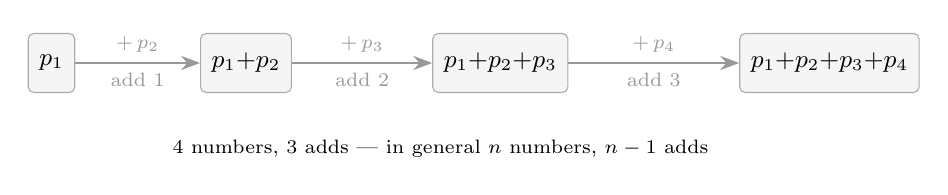
\begin{tikzpicture}[scale=0.95]
  \node[opbox] (p1) at (0,0)   {$p_1$};
  \node[opbox] (p2) at (2.6,0) {$p_1{+}p_2$};
  \node[opbox] (p3) at (6.0,0) {$p_1{+}p_2{+}p_3$};
  \node[opbox] (p4) at (10.4,0){$p_1{+}p_2{+}p_3{+}p_4$};
  \draw[opar] (p1) -- (p2) node[midway,above,font=\scriptsize]{$+\,p_2$}
                           node[midway,below,font=\scriptsize]{add 1};
  \draw[opar] (p2) -- (p3) node[midway,above,font=\scriptsize]{$+\,p_3$}
                           node[midway,below,font=\scriptsize]{add 2};
  \draw[opar] (p3) -- (p4) node[midway,above,font=\scriptsize]{$+\,p_4$}
                           node[midway,below,font=\scriptsize]{add 3};
  \node[font=\scriptsize] at (5.2,-1.15)
        {$4$ numbers, $3$ adds --- in general $n$ numbers, $n-1$ adds};
\end{tikzpicture}
\end{center}

\noindent So the dot product runs in two stages:

\begin{center}
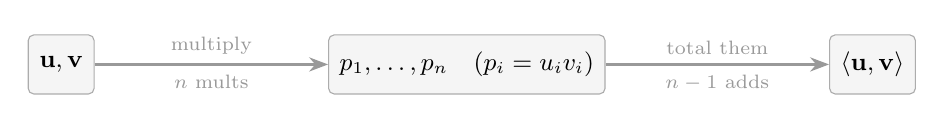
\begin{tikzpicture}[scale=0.92]
  \node[opbox] (a) at (0,0)    {$\vc{u},\vc{v}$};
  \node[opbox] (b) at (5.6,0)  {$p_1,\dots,p_n$ \ \ ($p_i=u_iv_i$)};
  \node[opbox] (c) at (11.2,0) {$\langle\vc{u},\vc{v}\rangle$};
  \draw[opar] (a) -- (b) node[midway,above,font=\scriptsize]{multiply}
                         node[midway,below,font=\scriptsize]{$n$ mults};
  \draw[opar] (b) -- (c) node[midway,above,font=\scriptsize]{total them}
                         node[midway,below,font=\scriptsize]{$n-1$ adds};
\end{tikzpicture}
\end{center}

\noindent Adding the two stages,
\[
  \boxed{\,\langle\vc{u},\vc{v}\rangle \text{ costs } n + (n-1) = 2n-1
          \text{ operations}\,}
\]

%------------------------------------------------------------------------------
\subsection{The norm}
%------------------------------------------------------------------------------
Next, $\norm{\vc{u}}$. Written out term by term,
\[
  \norm{\vc{u}} = \bigl(u_1^{2} + u_2^{2} + \cdots + u_n^{2}\bigr)^{1/2} .
\]
Now three stages. Each $u_i^{2}$ is the product $u_i\cdot u_i$, so squaring all
$n$ coordinates is $n$ mults. Totalling those $n$ squares is $n-1$ adds, by the
counting argument of \S1.3. And finally one square root is taken, of a single
scalar --- one operation, no matter how large $n$ is, because by that point only
one number is left.

\begin{center}
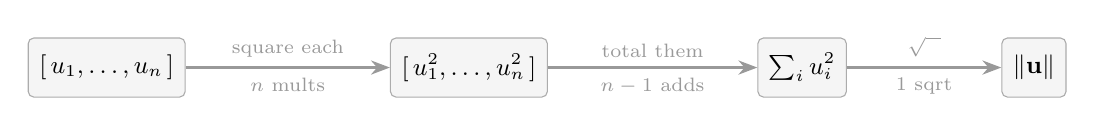
\begin{tikzpicture}[scale=0.92]
  \node[opbox] (a) at (0,0)    {$[\,u_1,\dots,u_n\,]$};
  \node[opbox] (b) at (5.0,0)  {$[\,u_1^{2},\dots,u_n^{2}\,]$};
  \node[opbox] (c) at (9.6,0)  {$\sum_i u_i^{2}$};
  \node[opbox] (d) at (12.8,0) {$\norm{\vc{u}}$};
  \draw[opar] (a) -- (b) node[midway,above,font=\scriptsize]{square each}
                         node[midway,below,font=\scriptsize]{$n$ mults};
  \draw[opar] (b) -- (c) node[midway,above,font=\scriptsize]{total them}
                         node[midway,below,font=\scriptsize]{$n-1$ adds};
  \draw[opar] (c) -- (d) node[midway,above,font=\scriptsize]{$\sqrt{\ \ }$}
                         node[midway,below,font=\scriptsize]{$1$ sqrt};
\end{tikzpicture}
\end{center}

\noindent Adding the three stages,
\[
  \boxed{\,\norm{\vc{u}} \text{ costs } n + (n-1) + 1 = 2n
          \text{ operations}\,}
\]

\begin{rmk}
It is worth noticing where the $1$ sits. The square root is applied \emph{once},
at the very end, to a scalar --- not once per coordinate. Miscounting this is
the most common error in a first operation count: the stages of a computation
operate on different numbers of quantities, and you must track how many are
still in play at each stage.
\end{rmk}

%------------------------------------------------------------------------------
\subsection{The projection}
%------------------------------------------------------------------------------
Now something with several moving parts. Recall from the vector unit, \S12.4,
\[
  \proj{\vc{u}}{\vc{v}}
  = \frac{\langle\vc{u},\vc{v}\rangle}{\norm{\vc{u}}}\cdot
    \frac{\vc{u}}{\norm{\vc{u}}} .
\]
The hard work is already done: we know what a dot product and a norm cost. What
remains is to take the formula apart and add up the pieces, being careful at
each step about whether the quantity involved is a scalar or a vector.

\begin{enumerate}[label=\textbf{\arabic*.},leftmargin=2.4em,itemsep=4pt,
                  topsep=4pt]
  \item $\langle\vc{u},\vc{v}\rangle$ --- a dot product, so $2n-1$ operations.
  \item $\norm{\vc{u}}$ --- a norm, so $2n$ operations. The formula asks for it
        \emph{twice}, once in each factor, so as written that is $4n$.
  \item $\langle\vc{u},\vc{v}\rangle/\norm{\vc{u}}$ --- careful here. Both of
        these are \emph{scalars}, so this is a single scalar division:
        $1$ operation.
  \item $\vc{u}/\norm{\vc{u}}$ --- here $\vc{u}$ is a \emph{vector}, and
        dividing it by a scalar is componentwise. That is $n$ divisions, so $n$
        operations.
  \item Finally the scalar from step 3 multiplies the vector from step 4, again
        componentwise: $n$ mults, so $n$ operations.
\end{enumerate}

\noindent Adding them up,
\[
  (2n-1) + 4n + 1 + n + n = 8n ,
\]
so the formula \emph{as written} costs $8n$ operations.

%------------------------------------------------------------------------------
\subsection{Doing it better}
%------------------------------------------------------------------------------
Is there anything wrong with that count? Mathematically, no --- $8n$ is the
honest cost of evaluating the expression exactly as it appears. But to anyone
who has written code, the problem is glaring.

\subsubsection*{First saving: stop computing the same thing twice}
Why did we compute $\norm{\vc{u}}$ \emph{twice}? The two occurrences are the
same number. Compute it once, keep it, and use it in both places. That deletes
one of the two $2n$ charges:
\[
  (2n-1) + 2n + 1 + n + n = 6n .
\]
Nothing about the mathematics changed --- only the bookkeeping. This is the
single most common optimisation there is, and it has a name in programming:
\emph{common subexpression elimination}.

\subsubsection*{Second saving: do not take a square root you are going to square}
Look at what $\norm{\vc{u}}$ is used for. It appears twice, and both times it
divides --- so what the formula really uses is $\norm{\vc{u}}^{2}$. And by the
vector unit's \S11.6,
\[
  \norm{\vc{u}}^{2} = \langle\vc{u},\vc{u}\rangle ,
\]
which is a dot product: $2n-1$ operations, with \emph{no square root at all}.
Rewriting the projection in the equivalent form already given in \S12.4,
\[
  \proj{\vc{u}}{\vc{v}}
  = \frac{\langle\vc{u},\vc{v}\rangle}{\norm{\vc{u}}^{2}}\,\vc{u} ,
\]
the count becomes
\[
  \underbrace{(2n-1)}_{\langle\vc{u},\vc{v}\rangle}
  + \underbrace{(2n-1)}_{\langle\vc{u},\vc{u}\rangle}
  + \underbrace{1}_{\text{one scalar division}}
  + \underbrace{n}_{\text{scale }\vc{u}}
  \;=\; 5n-1 .
\]

\noindent Notice the third saving hiding in that line. The old version made two
separate passes over $\vc{u}$ --- dividing by the norm, then multiplying by the
scalar --- costing $n+n$. Combining the two scalars into one \emph{before}
touching the vector reduces that to a single pass of $n$ mults.

\begin{center}
\renewcommand{\arraystretch}{1.35}
\begin{tabular}{@{}l l l@{}}
\toprule
\textbf{Version} & \textbf{Cost} & \textbf{What changed} \\
\midrule
As written                    & $8n$    & --- \\
Reuse $\norm{\vc{u}}$          & $6n$    & compute the norm once, not twice \\
Use $\norm{\vc{u}}^{2}=\langle\vc{u},\vc{u}\rangle$
                              & $5n-1$  & no square root; one pass over $\vc{u}$ \\
\bottomrule
\end{tabular}
\end{center}

\noindent For $n=1000$ that is $8000$ operations against $4999$ --- the same
answer, at a little over half the cost. And the square root, which we noted in
\S1.2 is among the slowest operations available, has been removed entirely.

%------------------------------------------------------------------------------
\subsection{Why count at all}
%------------------------------------------------------------------------------
A fair question at this point is why any of this matters. The formulas are
correct either way, and a modern machine will evaluate all three versions
faster than you can notice.

The reason is that we are stepping out of mathematics and into computation.
Until now every object in this course has been exact and every operation free:
$\R^{n}$ is infinite, a real number carries infinitely many digits, and writing
$\norm{\vc{u}}$ costs nothing because writing is not computing. A machine has
none of that. It has finitely many digits per number, finitely many operations
per second, and finite memory, and every one of those limits will eventually
bind.

The computations here are small, and modern hardware and libraries are heavily
optimised for exactly them. But the habit is what matters: taking a formula
apart, asking what each stage costs, and noticing when the same quantity is
being computed twice. Do that on a projection and you save a square root. Do it
on an algorithm that runs a projection a million times inside a loop, and the
difference is the difference between a program that finishes and one that does
not.

\lookahead Two threads start here. First, we have been counting \emph{exactly},
producing answers like $5n-1$; usually the constants and the $-1$ do not matter
and only the growth rate does, which is what \emph{asymptotic} notation captures
--- the reason $5n-1$ and $8n$ are ``the same'' in a sense worth making precise.
Second, we have assumed a machine stores real numbers. It does not; it stores
\emph{floating-point} numbers, of which there are finitely many, and arithmetic
on them is not quite the arithmetic of $\R$. Both are next.

%------------------------------------------------------------------------------
\subsection{Exercises}
%------------------------------------------------------------------------------
In each case, count the operations required, and keep the count \emph{as low as
possible} --- part of the exercise is noticing what the given information lets
you skip.

\begin{enumerate}[label=\textbf{E\arabic*.},leftmargin=2.8em,itemsep=7pt,
                  topsep=6pt]
  \item Let $\vc{u},\vc{v}\in\R^{200}$ be orthonormal. Count the operations
        needed to compute $\proj{\vc{u}}{\vc{v}}$.
  \item Let $\vc{u},\vc{v}\in\R^{50}$ with $\cos(\vc{u},\vc{v})=1$. Count the
        operations needed to compute $\norm{\vc{u}-\vc{v}}$.
  \item Let $\vc{u},\vc{v}\in\R^{25}$ be nonzero and linearly dependent. Count
        the operations needed to compute $\cos(\vc{u},\vc{v})$.
\end{enumerate}

\subsubsection*{Answer key}

\noindent\textbf{E1.} \emph{Zero operations.} ``Orthonormal'' means both vectors
are unit length \emph{and} orthogonal, so $\langle\vc{u},\vc{v}\rangle=0$ is
given. Then
\[
  \proj{\vc{u}}{\vc{v}}
  = \frac{\langle\vc{u},\vc{v}\rangle}{\norm{\vc{u}}^{2}}\,\vc{u}
  = \frac{0}{1}\,\vc{u} = \vc{0},
\]
and the answer is the zero vector, written down without arithmetic. Ignoring the
hypothesis and evaluating the optimised formula would have cost $5n-1=999$
operations to arrive at the same $\vc{0}$. The lesson is that recognising
structure beats computing.

\smallskip
\noindent\textbf{E2.} \emph{$3n=150$ operations, and the hypothesis does not
help.} Directly: $\vc{u}-\vc{v}$ costs $n=50$ subtractions, and taking the norm
of the result costs $2n=100$, for $3n=150$ in total.

It is worth seeing why the given information is no use. Since
$\cos(\vc{u},\vc{v})=1$ the two vectors point the same way, and expanding as in
the vector unit's \S13 gives
$\norm{\vc{u}-\vc{v}}^{2}
 =\norm{\vc{u}}^{2}-2\langle\vc{u},\vc{v}\rangle+\norm{\vc{v}}^{2}
 =\bigl(\norm{\vc{u}}-\norm{\vc{v}}\bigr)^{2}$,
so $\norm{\vc{u}-\vc{v}}=\bigl\lvert\norm{\vc{u}}-\norm{\vc{v}}\bigr\rvert$.
That is a genuine shortcut in appearance, but it costs two norms and a
subtraction: $2n+2n+1=4n+1=201$, which is \emph{more} than $150$. A shortcut is
only a shortcut if it is cheaper.

\smallskip
\noindent\textbf{E3.} \emph{$1$ operation.} Linearly dependent and nonzero means
parallel (vector unit, \S18.4), so $\vc{v}=\alpha\vc{u}$ for some
$\alpha\neq0$, and the angle between them is $0$ or $\pi$. Hence
$\cos(\vc{u},\vc{v})=\pm1$, with the sign being the sign of $\alpha$. To find
that sign, pick any index $i$ with $u_i\neq0$ and form $\alpha=v_i/u_i$: one
division. Then $\cos(\vc{u},\vc{v})=+1$ if $\alpha>0$ and $-1$ if $\alpha<0$.

Evaluating the definition instead would cost one dot product, two norms, one
mult and one division: $(2n-1)+2n+2n+1+1=6n+1=151$.

%==============================================================================
\section{How costs scale: asymptotic analysis}
%==============================================================================
Section~1 produced exact counts: $n$, $2n-1$, $2n$, $5n-1$. Exactness is
satisfying but it is rarely what we want to know. In computer science the
question is almost always how the count \emph{scales} --- what happens to the
cost as the input grows.

%------------------------------------------------------------------------------
\subsection{What an algorithm is}
%------------------------------------------------------------------------------
\begin{defn}[Algorithm, informally]
An \textbf{algorithm} is a finite sequence of steps aimed at solving a problem.
It usually has an \textbf{input} and always produces an \textbf{output}.
\end{defn}

\noindent Vector addition is about as simple an algorithm as exists. Its input
is the pair $\vc{u},\vc{v}\in\R^{n}$; its steps are the $n$ componentwise adds;
its output is the vector $\vc{w}=\vc{u}+\vc{v}$.

\begin{rmk}
Every algorithm emits an output --- an algorithm that produced nothing would
have solved nothing. An input, though, is optional: an algorithm that prints the
first thousand primes takes no input at all, and simply runs.
\end{rmk}

%------------------------------------------------------------------------------
\subsection{Operation count as a function of input size}
%------------------------------------------------------------------------------
To speak about scaling we need to say what is growing. For an algorithm on
vectors, the \textbf{input size} is the number of components, $n$. So write the
operation count as a function of it:
\[
  f(n) = n ,
\]
where $n$ is the number of components and $f(n)$ is the exact number of
operations vector addition performs. Note that $n$ ranges over the natural
numbers --- an input size is a count, and there is no vector in $\R^{2.7}$ ---
so the graph of $f$ is a set of isolated points, not a curve.

\begin{center}
\begin{tikzpicture}[xscale=0.82,yscale=0.72]
  \draw[axisline] (0,0) -- (9.0,0) node[right,font=\scriptsize,black]{$n$};
  \draw[axisline] (0,0) -- (0,10.4) node[above,font=\scriptsize,black]{operations};
  % ticks drawn top-to-bottom / right-to-left so the label lands clear of them
  \foreach \n in {2,4,6,8} { \draw[gray!70] (\n,0.16) -- (\n,-0.16)
        node[below=1pt,font=\scriptsize,gray]{$\n$}; }
  \foreach \y in {2,4,6,8,10} { \draw[gray!70] (0.13,\y) -- (-0.13,\y)
        node[left=1pt,font=\scriptsize,gray]{$\y$}; }
  \draw[RoyalBlue,dotted,thick] (1,1) -- (8,8);
  \foreach \n in {1,...,8} { \fill[RoyalBlue] (\n,\n) circle (2.4pt); }
  \node[right,font=\scriptsize,RoyalBlue] at (8.15,8) {$f(n)=n$};
\end{tikzpicture}
\end{center}

\noindent The dotted line is interpolation, drawn only so the eye can see the
pattern; the algorithm exists only at the dots. That pattern --- the relative
geometry of $f$ --- is what we mean by the \textbf{scale} of the algorithm, and
here it is plainly \emph{linear}. The number of operations vector addition
performs scales linearly with the number of components.

%------------------------------------------------------------------------------
\subsection{The other algorithms}
%------------------------------------------------------------------------------
We already have counts for three more. Writing each as a function of input size:
\[
  \underbrace{g(n)=2n}_{\norm{\vc{u}}},
  \qquad
  \underbrace{h(n)=2n-1}_{\langle\vc{u},\vc{v}\rangle},
  \qquad
  \underbrace{\ell(n)=5n-1}_{\proj{\vc{u}}{\vc{v}}\ \text{computed efficiently}} .
\]

\begin{center}
\begin{tikzpicture}[xscale=1.05,yscale=0.28]
  \draw[axisline] (0,0) -- (8.8,0) node[right,font=\scriptsize,black]{$n$};
  \draw[axisline] (0,0) -- (0,44) node[above,font=\scriptsize,black]{operations};
  \foreach \n in {2,4,6,8} { \draw[gray!70] (\n,0.55) -- (\n,-0.55)
        node[below=1pt,font=\scriptsize,gray]{$\n$}; }
  \foreach \y in {10,20,30,40} { \draw[gray!70] (0.09,\y) -- (-0.09,\y)
        node[left=1pt,font=\scriptsize,gray]{$\y$}; }
  \draw[BrickRed,dotted,thick]    (1,4)  -- (8,39);
  \draw[ForestGreen,dotted,thick] (1,2)  -- (8,16);
  \draw[Orange,dotted,thick]      (1,1)  -- (8,15);
  \draw[RoyalBlue,dotted,thick]   (1,1)  -- (8,8);
  \foreach \n in {1,...,8} {
    \fill[BrickRed]    (\n,{5*\n-1}) circle (2.4pt);
    \fill[ForestGreen] (\n,{2*\n})   circle (2.4pt);
    \fill[Orange]      (\n,{2*\n-1}) circle (2.4pt);
    \fill[RoyalBlue]   (\n,\n)       circle (2.4pt);
  }
  \node[right,font=\scriptsize,BrickRed]    at (8.1,39) {$\ell(n)=5n-1$};
  \node[right,font=\scriptsize,ForestGreen] at (8.1,17.5) {$g(n)=2n$};
  \node[right,font=\scriptsize,Orange]      at (8.1,13.5) {$h(n)=2n-1$};
  \node[right,font=\scriptsize,RoyalBlue]   at (8.1,8)  {$f(n)=n$};
\end{tikzpicture}
\end{center}

\noindent What do the four have in common? Every one of them is a straight line.
The slopes differ and one is shifted down by $1$, but the \emph{shape} is
identical: all four algorithms scale linearly with the number of components.
Make the input as large as you like and that does not change --- a line stays a
line.

%------------------------------------------------------------------------------
\subsection{Big-O notation}
%------------------------------------------------------------------------------
Since the shape is what matters and the constants are not, we want notation that
records the shape and discards the rest.

\begin{quote}
For a count that scales linearly in the long run we write $O(n)$, read
``big-oh of $n$'', and call it the algorithm's \textbf{runtime complexity} ---
also its \textbf{asymptotic runtime} or \textbf{time complexity}.
\end{quote}

\noindent So vector addition is $O(n)$. And so are the norm, the dot product,
and the projection, despite their different constants and shifts. Big-O is
concerned only with the underlying scale, which is set by the \textbf{dominant
term} of the count.

\begin{warn}[We are not measuring time]
``Time complexity'' is a misleading name, and it is worth being clear about it
early. We are counting \emph{operations}, not seconds. How long a program
actually takes depends on the processor, the language, the compiler, how the
data sits in memory, and what else the machine is doing --- two $O(n)$
implementations can easily differ by a factor of a hundred in wall-clock time.
What Big-O describes is how the operation count \emph{grows}, and that is a
property of the algorithm rather than of any machine that runs it.
\end{warn}

%------------------------------------------------------------------------------
\subsection{Finding the dominant term}
%------------------------------------------------------------------------------
For a polynomial count the dominant term is the highest-degree one. Suppose an
algorithm's count is modelled by
\[
  f(n) = 3n^{2} + 2n + 3 .
\]
As $n$ grows, $3n^{2}$ outpaces $2n$ and $3$ so completely that they stop
mattering, and the coefficient $3$ does not change the shape --- a parabola
stretched is still a parabola. So $f$ scales quadratically and we write
$f(n)$ is $O(n^{2})$.

When the terms are not both polynomials it can be less obvious which one wins,
and a table of values helps.

\begin{ex}[A table that nearly misleads]
Consider $f(n) = 2^{n} + n^{5}$.

\begin{center}
\renewcommand{\arraystretch}{1.25}
\begin{tabular}{@{}r r r l@{}}
\toprule
$n$ & $2^{n}$ & $n^{5}$ & larger \\
\midrule
$1$  & $2$             & $1$          & $2^{n}$ \\
$2$  & $4$             & $32$         & $n^{5}$ \\
$5$  & $32$            & $3{,}125$    & $n^{5}$ \\
$10$ & $1{,}024$       & $100{,}000$  & $n^{5}$ \\
$15$ & $32{,}768$      & $759{,}375$  & $n^{5}$ \\
$20$ & $1{,}048{,}576$ & $3{,}200{,}000$ & $n^{5}$ \\
$22$ & $4{,}194{,}304$ & $5{,}153{,}632$ & $n^{5}$ \\
$23$ & $8{,}388{,}608$ & $6{,}436{,}343$ & $\mathbf{2^{n}}$ \\
$25$ & $33{,}554{,}432$ & $9{,}765{,}625$ & $2^{n}$ \\
$30$ & $1{,}073{,}741{,}824$ & $24{,}300{,}000$ & $2^{n}$ \\
\bottomrule
\end{tabular}
\end{center}

\noindent Read only the first six rows and you would conclude that $n^{5}$
dominates. It does not. The two cross between $n=22$ and $n=23$, and past that
$2^{n}$ pulls away without limit --- by $n=30$ it is more than forty times
larger, and the gap keeps widening. So the dominant term is $2^{n}$, and
\[
  f(n) = 2^{n}+n^{5} \quad\text{is}\quad O(2^{n}) .
\]
\end{ex}

\begin{warn}
That example is the reason a table of values is a hint and not a proof. An
exponential eventually beats every polynomial, no matter how large the
polynomial's degree --- but ``eventually'' can be far to the right of where you
stopped looking. Big-O is a statement about the long run, so a handful of small
values can point the wrong way.
\end{warn}

\begin{rmk}[A tip: compare with a ratio]
A quick way to settle which of two positive functions dominates is to look at
their ratio as $n$ grows. If
\[
  \lim_{n\to\infty}\frac{f(n)}{g(n)} = 0 ,
\]
then $f$ is negligible against $g$, so $g$ is the dominant one; if the limit is
$\infty$, then $f$ dominates; and if it is a positive constant, the two scale
alike. Two standard facts from Calculus~I settle most cases immediately:
exponentials outgrow all polynomials, and all polynomials outgrow logarithms.
For the example above, $n^{5}/2^{n}\to0$, confirming $2^{n}$ as dominant without
any table.
\end{rmk}

%------------------------------------------------------------------------------
\subsection{Complexities you will meet}
%------------------------------------------------------------------------------
A few growth rates account for most algorithms in practice.

\begin{center}
\renewcommand{\arraystretch}{1.3}
\begin{tabular}{@{}l l@{}}
\toprule
\textbf{Complexity} & \textbf{A typical algorithm} \\
\midrule
$O(1)$          & reading one entry of a vector \\
$O(\log_2 n)$   & binary search in a sorted index \\
$O(n)$          & vector addition, the dot product, the norm \\
$O(n\log_2 n)$  & a good general-purpose sort \\
$O(n^{2})$      & a naive sort; a matrix--vector product \\
$O(n^{3})$      & naive matrix multiplication; Gaussian elimination \\
$O(2^{n})$      & checking every subset of $n$ items \\
\bottomrule
\end{tabular}
\end{center}

\begin{center}
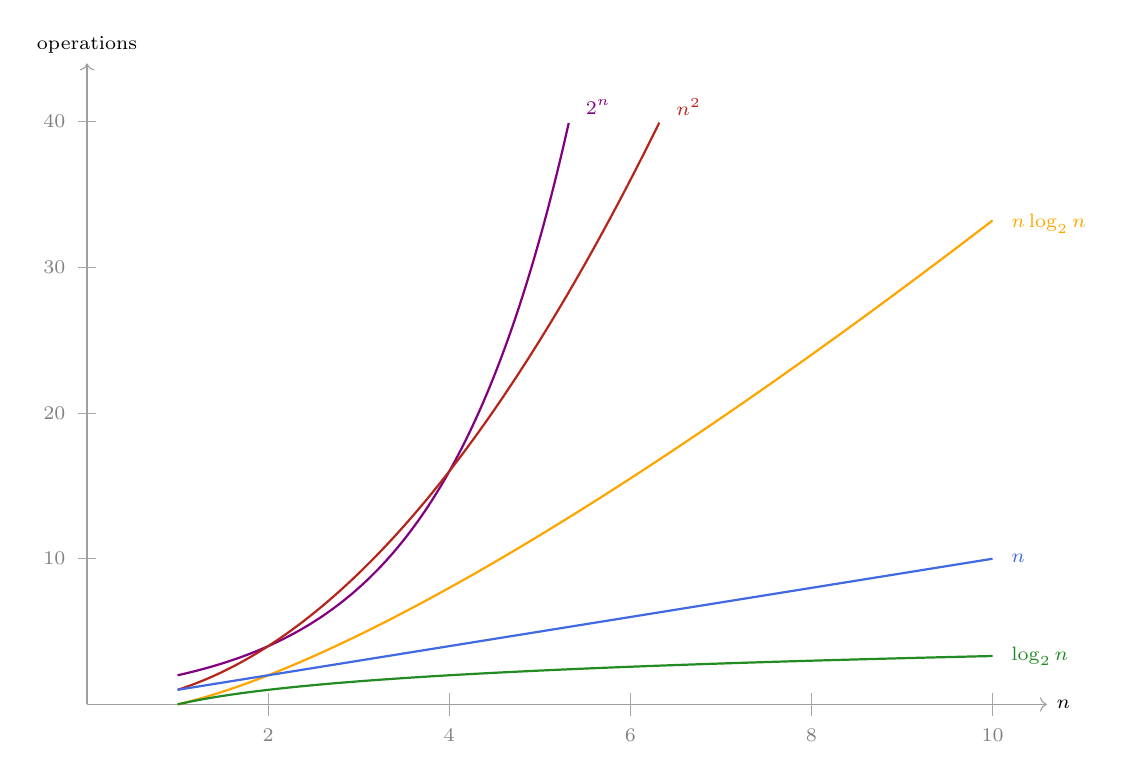
\begin{tikzpicture}[xscale=1.15,yscale=0.185]
  \draw[axisline] (0,0) -- (10.6,0) node[right,font=\scriptsize,black]{$n$};
  \draw[axisline] (0,0) -- (0,44) node[above,font=\scriptsize,black]{operations};
  \foreach \n in {2,4,6,8,10} { \draw[gray!70] (\n,0.8) -- (\n,-0.8)
        node[below=1pt,font=\scriptsize,gray]{$\n$}; }
  \foreach \y in {10,20,30,40} { \draw[gray!70] (0.1,\y) -- (-0.1,\y)
        node[left=1pt,font=\scriptsize,gray]{$\y$}; }
  \draw[Purple,thick,domain=1:5.32,smooth,variable=\x,samples=60]
        plot ({\x},{2^\x});
  \draw[BrickRed,thick,domain=1:6.32,smooth,variable=\x,samples=60]
        plot ({\x},{\x*\x});
  \draw[Orange,thick,domain=1:10,smooth,variable=\x,samples=60]
        plot ({\x},{\x*ln(\x)/ln(2)});
  \draw[RoyalBlue,thick,domain=1:10,smooth,variable=\x,samples=60]
        plot ({\x},{\x});
  \draw[ForestGreen,thick,domain=1:10,smooth,variable=\x,samples=60]
        plot ({\x},{ln(\x)/ln(2)});
  \node[right,font=\scriptsize,Purple]      at (5.4,41)  {$2^{n}$};
  \node[right,font=\scriptsize,BrickRed]    at (6.4,41)  {$n^{2}$};
  \node[right,font=\scriptsize,Orange]      at (10.1,33) {$n\log_2 n$};
  \node[right,font=\scriptsize,RoyalBlue]   at (10.1,10) {$n$};
  \node[right,font=\scriptsize,ForestGreen] at (10.1,3.3){$\log_2 n$};
\end{tikzpicture}
\end{center}

\noindent The vertical spread at the right-hand edge is the whole point. At
$n=10$ the logarithm has reached about $3$ while $2^{n}$ passed $40$ before
$n$ even reached $6$. Choosing a better algorithm is not a small optimisation
like the ones in \S1.6; it changes which problems are solvable at all.

%------------------------------------------------------------------------------
\subsection{The formal definition}
%------------------------------------------------------------------------------
Everything so far has been informal --- ``dominant term'', ``in the long run''.
Here is the precise statement.

\begin{defn}[Big-O]
For functions $f$ and $g$, we say $f(n)$ is $O\bigl(g(n)\bigr)$ if and only if
there exist constants $C>0$ and $n_0\ge0$ such that
\[
  \lvert f(n)\rvert \;\le\; C\,\bigl\lvert g(n)\bigr\rvert
  \qquad\text{for all } n\ge n_0 .
\]
\end{defn}

\noindent Every function we will use counts operations, so all of them are
positive, and the absolute values may be dropped:
\[
  f(n) \le C\,g(n) \qquad\text{for all } n\ge n_0 .
\]
Read the definition as licensing two concessions. The constant $C$ says we do
not care about a fixed multiplicative factor; the threshold $n_0$ says we do not
care what happens for small inputs. Proving $f$ is $O(g)$ therefore amounts to
\emph{exhibiting} a $C$ large enough and an $n_0$ far enough right that the
inequality holds from there on. You do not need the smallest such $C$ --- any
one that works will do.

%------------------------------------------------------------------------------
\subsection{Three proofs}
%------------------------------------------------------------------------------
\begin{ex}
Show that $f(n)=2n^{2}+2n$ is $O(n^{2})$.

For every $n\ge1$ we have $n\le n^{2}$, hence $2n\le 2n^{2}$, and so
\[
  f(n) = 2n^{2}+2n \;\le\; 2n^{2}+2n^{2} = 4n^{2} .
\]
Take $C=4$ and $n_0=1$. \hfill$\blacksquare$
\end{ex}

\begin{ex}
Show that $f(n)=n^{4}+n^{3}$ is $O(n^{4})$.

For every $n\ge1$ we have $n^{3}\le n^{4}$, so
\[
  f(n) = n^{4}+n^{3} \;\le\; n^{4}+n^{4} = 2n^{4} .
\]
Take $C=2$ and $n_0=1$. \hfill$\blacksquare$
\end{ex}

\noindent Both follow the same recipe: bound every lower-order term by the
dominant one, then collect. That recipe handles any polynomial.

\begin{ex}[Challenge]
Show that $1^{2}+2^{2}+3^{2}+\cdots+n^{2}$ is $O(n^{3})$.

Here there is no highest-degree term to bound against, because the number of
terms itself grows with $n$. The trick is to bound each term by the largest one.
Every index $k$ in the sum satisfies $k\le n$, hence $k^{2}\le n^{2}$; and there
are exactly $n$ terms. Therefore
\[
  \sum_{k=1}^{n}k^{2}
  \;\le\; \underbrace{n^{2}+n^{2}+\cdots+n^{2}}_{n\ \text{terms}}
  \;=\; n\cdot n^{2} = n^{3} .
\]
Take $C=1$ and $n_0=1$. \hfill$\blacksquare$
\end{ex}

%------------------------------------------------------------------------------
\subsection{A note on what Big-O does and does not say}
%------------------------------------------------------------------------------
Complexity notation comes in several forms. Big-O is an \emph{upper} bound on
growth --- it says the cost is no worse than a certain shape. There are
companions for the other directions: $\Omega$ for a lower bound, and $\Theta$
when upper and lower bounds match. For this course Big-O is enough.

\begin{rmk}
Big-O is often described loosely as ``the worst case'', and for our purposes
nothing goes wrong in saying so. Strictly, though, two separate ideas are being
run together. \emph{Worst, best} and \emph{average case} concern which
\emph{input} you measure; Big-O concerns how a count \emph{grows} once you have
chosen. One can perfectly well speak of an average-case $O(n\log_2 n)$.

For the algorithms in \S1 the distinction happens not to arise: vector addition
performs exactly $n$ adds whatever the entries happen to be, and the same holds
for the dot product, the norm and the projection. Their cost depends only on
$n$, so best, average and worst case coincide. Algorithms where they differ ---
searching, sorting, elimination with pivoting --- are where the vocabulary earns
its keep.
\end{rmk}

\noindent Big-O is ubiquitous well beyond this course: it is the common language
of software engineering, numerical analysis and scientific computing, and it is
how the cost of every algorithm in the rest of this unit will be reported.

\lookahead One assumption remains unexamined. Throughout \S1 and \S2 we have
counted operations on \emph{real numbers}, as though a machine could hold one.
It cannot: there are infinitely many reals and only finitely many patterns of
bits. What a computer actually stores is a \emph{floating-point} number, and
arithmetic on those is not quite the arithmetic of $\R$ --- sums can depend on
the order you add them, and quantities that should cancel exactly do not. That
is the next topic, and the last of this lecture.

%==============================================================================
\section{The set a computer actually works in}
%==============================================================================
%------------------------------------------------------------------------------
\subsection{Every subject starts with a set}
%------------------------------------------------------------------------------
Mathematical subjects share a structural pattern, and it is worth naming before
we disturb it. In each one there is a \emph{set} of objects and a collection of
\emph{operations} or rules that act on them. Everything else --- the questions,
the observations, the conjectures, the theorems --- grows out of asking what
happens to those objects under those rules in one scenario after another.

Calculus is a clear case. The underlying set is the real numbers, together with
functions built from them. The operations on functions are governed by
properties of $\R$, and out of those properties comes the limit; out of the
limit comes the derivative; and out of the derivative comes the rest of the
subject. Nothing in that chain was available until the set was fixed.

\begin{center}
\renewcommand{\arraystretch}{1.35}
\begin{tabular}{@{}l l l@{}}
\toprule
\textbf{Underlying set} & \textbf{Some operations} & \textbf{What grows from it} \\
\midrule
$\R$, and functions on it & limits, derivatives, integrals & calculus, real analysis \\
$\C$                      & complex arithmetic, conjugation & complex analysis \\
$\Z$                      & divisibility, congruence, counting & number theory, combinatorics \\
$\R^{n}$, later matrices  & addition, scaling, the dot product & linear algebra \\
\bottomrule
\end{tabular}
\end{center}

\noindent The underlying set plants the seed for a whole garden of mathematical
knowledge.

\begin{rmk}
The vector unit was exactly this pattern, carried out in front of you. We fixed
the set --- $\R^{2}$, later $\R^{n}$ --- then fixed the operations, and then
spent five parts asking what followed: when do two vectors span, when are they
independent, what does orthogonality buy, which subsets are closed. None of
those questions could even be \emph{stated} before the set and the operations
were on the table.
\end{rmk}

%------------------------------------------------------------------------------
\subsection{A computer works in a different set}
%------------------------------------------------------------------------------
Here is the disturbance. When a computer tackles a mathematical problem --- and
especially a \emph{continuous} one, a problem posed over the real numbers --- it
does not work in $\R$. It works in a peculiar set of its own.

\begin{defn}[Floating-point numbers, informally]
The \textbf{floating-point numbers}, written $\F$, are a \emph{finite} set of
numbers used to approximate the real numbers, each carrying only a fixed,
finite number of digits.
\end{defn}

\noindent Two consequences follow immediately, and both matter.

\begin{itemize}[leftmargin=1.4em,itemsep=4pt]
  \item $\F$ is \emph{finite}, while $\R$ is not merely infinite but
        uncountable. So $\F\subset\R$: every floating-point number is a real
        number, and almost no real number is a floating-point number. The
        machine is working inside a very sparse subset of the set the problem
        was posed in.
  \item The elements of $\F$ are \emph{not evenly spaced}. They crowd together
        near zero and spread apart as the magnitude grows, because a fixed
        number of digits buys finer resolution for small numbers than for large
        ones.
\end{itemize}

\noindent The picture below shows both facts at once. It uses a miniature
floating-point system --- three digits of precision in base $2$, with only four
exponents --- so that the whole set fits on the page; a real system has vastly
more points but is spaced in exactly this pattern.

\begin{center}
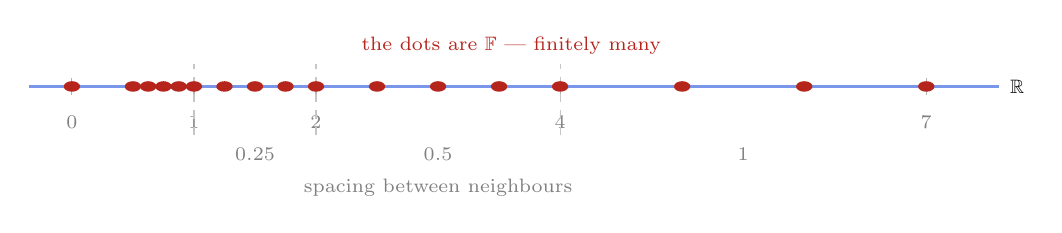
\begin{tikzpicture}[xscale=1.55,yscale=1]
  \draw[RoyalBlue!70,line width=1.1pt] (-0.35,0) -- (7.6,0)
        node[right,font=\scriptsize,black]{$\R$};
  % two label rows, kept well apart: axis values just under the line, and the
  % neighbour spacings lower down with their own caption
  \foreach \x/\lab in {0/0, 1/1, 2/2, 4/4, 7/7}
     { \draw[gray!60] (\x,0.11) -- (\x,-0.11);
       \node[below=4pt,font=\scriptsize,gray] at (\x,-0.11) {$\lab$}; }
  \draw[gray!45,dashed] (1,-0.62) -- (1,0.28);
  \draw[gray!45,dashed] (2,-0.62) -- (2,0.28);
  \draw[gray!45,dashed] (4,-0.62) -- (4,0.28);
  \foreach \x in {0, 0.5,0.625,0.75,0.875, 1,1.25,1.5,1.75,
                  2,2.5,3,3.5, 4,5,6,7}
     { \fill[BrickRed] (\x,0) circle (1.9pt); }
  \node[font=\scriptsize,BrickRed] at (3.6,0.52)
        {the dots are $\F$ --- finitely many};
  \node[font=\scriptsize,gray] at (1.5,-0.86) {$0.25$};
  \node[font=\scriptsize,gray] at (3,-0.86)   {$0.5$};
  \node[font=\scriptsize,gray] at (5.5,-0.86) {$1$};
  \node[font=\scriptsize,gray] at (3,-1.28)   {spacing between neighbours};
\end{tikzpicture}
\end{center}

\noindent Read the spacing across the picture: it \emph{doubles} at every power
of two. Between $1$ and $2$ the representable numbers are $0.25$ apart; between
$2$ and $4$ they are $0.5$ apart; between $4$ and $8$ they are $1$ apart. Near
zero they are packed tightly, and far from zero they are strewn thinly. The line
is continuous; the dots are all the machine has.

Everything in $\R$ that is not a dot must be \emph{rounded} to the nearest dot
before the machine can hold it. That rounding is small, and for a single number
it is harmless. The question --- which is what makes this a topic rather than a
footnote --- is what happens when millions of such roundings accumulate through
an algorithm like the ones we counted in \S1.

%------------------------------------------------------------------------------
\subsection{Floats and doubles}
%------------------------------------------------------------------------------
You have almost certainly met this set already. Programming languages expose it
directly, and name the members by their \textbf{precision} --- the number of
digits each one carries:

\begin{center}
\renewcommand{\arraystretch}{1.3}
\begin{tabular}{@{}l l l@{}}
\toprule
\textbf{Name} & \textbf{Storage} & \textbf{Roughly} \\
\midrule
\texttt{float}, single precision, \texttt{float32}
  & $32$ bits & about $7$ decimal digits \\
\texttt{double}, double precision, \texttt{float64}
  & $64$ bits & about $16$ decimal digits \\
\bottomrule
\end{tabular}
\end{center}

\noindent A \texttt{double} is the default nearly everywhere it matters: it is
what Python's \texttt{float} is, what MATLAB uses unless told otherwise, and
what numerical libraries assume. A \texttt{float} halves the storage and the
precision, which is a real trade in graphics and machine learning and a
liability almost everywhere else.

The word \emph{precision} is the one to hold on to. It does not mean the numbers
are approximately right in some vague sense; it means each one carries a
specific, countable number of digits, and everything past that is gone.

%------------------------------------------------------------------------------
\subsection{Base 2}
%------------------------------------------------------------------------------
One more ingredient before we can say what a floating-point number actually
\emph{is}. A classical computer stores everything --- numbers included --- as
patterns of $0$s and $1$s, which is to say in \textbf{binary}.

Binary is not exotic. It is simply a numerical \emph{base}, base $2$, and we
have been conditioned by a decade of schooling to think in base $10$ instead ---
for no better reason than that people have ten fingers. In any base $b$, a
string of digits is shorthand for a sum of multiples of powers of $b$:

\begin{center}
\renewcommand{\arraystretch}{1.35}
\begin{tabular}{@{}l l l@{}}
\toprule
& \textbf{Place values} & \textbf{Value} \\
\midrule
$237_{10}$  & $2(10^{2}) + 3(10^{1}) + 7(10^{0})$
            & $200+30+7 = 237$ \\
$1011_{2}$  & $1(2^{3}) + 0(2^{2}) + 1(2^{1}) + 1(2^{0})$
            & $8+0+2+1 = 11$ \\
\bottomrule
\end{tabular}
\end{center}

\noindent The same idea continues to the right of the point, with negative
powers:
\[
  0.101_{2}
  = 1\bigl(2^{-1}\bigr) + 0\bigl(2^{-2}\bigr) + 1\bigl(2^{-3}\bigr)
  = \tfrac12 + \tfrac18
  = 0.625 .
\]
So the toy system in the figure above was nothing more than this: a few binary
digits, scaled by a power of two.

\lookahead A base is a choice of bookkeeping, and normally an innocent one ---
$0.625$ is $0.625$ whether you write it in base $10$ or as $0.101_{2}$. But the
choice is not always innocent, because a fraction that terminates in one base
need not terminate in another. That is where the surprises live, and it is where
we pick up next.

\end{document}
